\chapter[Método]{Método}

O método utilizado é uma interpretação do processo proposto por \citeonline{fayyad1996data} para descoberta de conhecimento, onde o objetivo principal é mapear um grande volume de dados para formas mais compactas, abstratas ou úteis para se encontrar padrões\footnote{O termo padrão é utilizado neste trabalho para designar um padrão encontrado nos dados.} e extrair informação.

A \autoref{fig:processo} apresenta o processo no qual, a partir de um banco de dados de currículos Lattes, são obtidos indicadores em redes de coautoria inter- e intra-áreas que são analisados para determinar o impacto que uma área do conhecimento exerce em outra.

\begin{figure}[htpb]
  \centering
  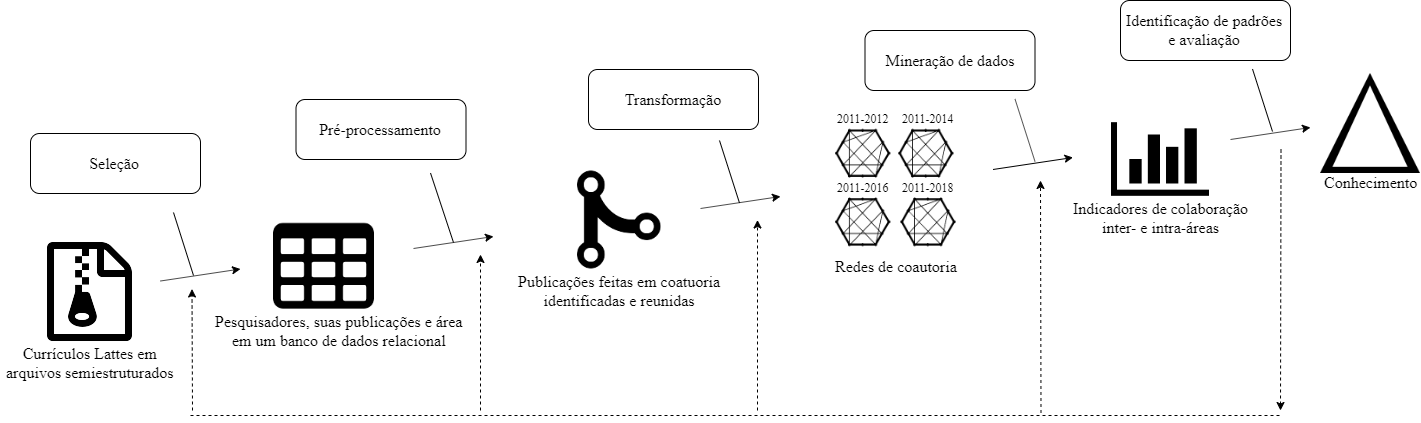
\includegraphics[scale=.3]{figuras/diagrama-fayyad}
  \caption{Uma visão geral das etapas adotadas no processo de descoberta de conhecimento.}
  \label{fig:processo}
\end{figure}

As etapas de seleção, pré-processamento e transformação preparam o banco de dados para a etapa de mineração de dados, onde algoritmos para extrair padrões são aplicados. Esses padrões são então interpretados e utilizados para gerar conhecimento.

\section{Seleção}

Os currículos Lattes em formato XML foram processados por um sistema onde as áreas de atuação e produção bibliográfica do pesquisador foram extraídas e armazenadas em um banco de dados relacional.

Neste trabalho os tipos de produção bibliográfica considerados são: publicações completas em periódicos, publicações completas em conferências, capítulos de livros publicados e livros publicados, os quais são referenciados como publicações científicas.
d
A \autoref{fig:er} apresenta o modelo entidade-relacionamento que descreve os pesquisadores atuando em múltiplas áreas do conhecimento e escrevendo múltiplas publicações científicas.

\begin{figure}[htpb]
  \centering
  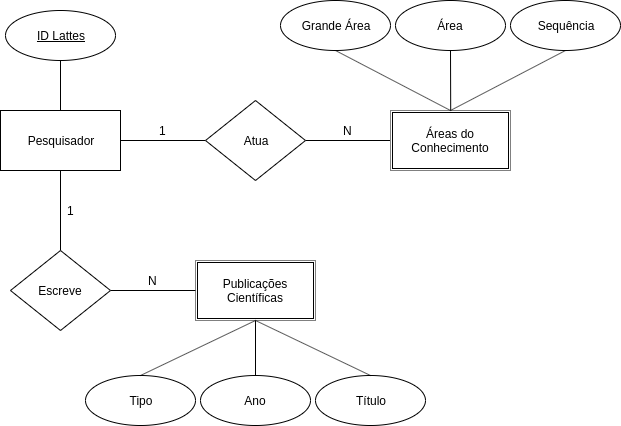
\includegraphics[scale=.5]{figuras/diagrama-er}
  \caption{Modelo entidade-relacionamento descrevendo as relações entre o pesquisador, suas áreas de atuação e suas publicações científicas.}
  \label{fig:er}
\end{figure}

\section{Pré-processamento}

Diversas produções científicas nessa área \cite{franceschet2011collaboration} \cite{mena2013prospecccao} \cite{reuther2006managing} descrevem casos onde uma publicação têm diversos nomes (sinônimos) e casos onde diferentes publicações possuem o mesmo nome (homônimos), cujos requerem tratamento a fim de obter um resultado mais confiável na etapa seguinte.

Publicações sinônimas acontecem neste trabalho porque existem diferentes títulos para uma mesma publicação que estão cadastrados no currículo Lattes dos pesquisadores envolvidos. A (colocar tabela) apresenta casos onde houve abreviação de palavras, omissão de pontuação ou erros de digitação.

ComoPara este cenário foi proposto o \autoref{alg:normalizacao}, que normaliza os títulos das publicações removendo diacríticos\footnote{Um diacrítico é um sinal gráfico que se coloca sobre, sob ou através de uma letra para alterar a sua realização fonética, isto é, o seu som, ou para marcar qualquer outra característica linguística.} e elementos que não pertencem ao título identificados no decorrer deste trabalho, como tags de marcação de hipertexto e caracteres com codificação HTML.

\begin{algorithm}
\caption{Normalização do título de publicações}
\label{alg:normalizacao}
\begin{algorithmic}[1]

\Procedure{NormalizeTitulo}{titulo}
\State $titulo\gets \Call{DecodifiqueCaracteresHtml}{titulo}$
\State $titulo\gets \Call{ExtraiaConteudoDaTagCDATA}{titulo}$
\State $titulo\gets \Call{RemovaMarcacaoDeHipertexto}{titulo}$
\State $titulo\gets \Call{NormalizeParaAFormaNFKD}{titulo}$
\State $titulo\gets \Call{RemovaDiacriticosDeCaracteresASCII}{titulo}$
\State $titulo\gets \Call{NormalizeParaAFormaNFC}{titulo}$
\State \Return $titulo$
\EndProcedure

\end{algorithmic}
\end{algorithm}

Publicações homônimas são mais difíceis de ocorrer pois serão comparadas apenas publicações de um mesmo tipo referentes a um mesmo ano. Ainda, para haver o casamento entre publicações, é necessário que os títulos tenham pelo menos 3 palavras, para evitar que editoriais, por exemplo, sejam considerados uma coautoria.

Caso publicações homônimas não sejam identificadas corretamente será possível observar que a lista de coautores de um autor se dividirá em dois ou mais grupos altamente interconectados, mas sem colaborações entre grupos diferentes \cite{franceschet2011collaboration}. Ao detectar casos como este, poderá ser realizado tratamento manual.

\section{Transformação}

Usando as publicações obtidas nos currículos Lattes é possível identificar dois pesquisadores como coautores se uma mesma publicação aparece em seus currículos, e com isso construir uma rede de coautoria onde os nós são pesquisadores e os vértices a coautoria entre eles. O mesmo procedimento pode ser feito por períodos (\textit{e.g.}, biênio ou triênio), onde se obtém uma série de redes de coautoria com espaçamento temporal.

Para identificar as coautorias entre quaisquer dois autores foi proposto o \autoref{alg:coautoria}, que compara todas as publicações dentro de um mesmo ano usando o algoritmo de distância Levenshtein (\autoref{alg:levenshtein}).

Atribuímos a área do conhecimento do pesquisador a cada uma de suas publicações. Assim, com as coautorias identificadas temos também a colaboração entre as áreas. Cada interação entre áreas em uma publicação única conta apenas uma vez, assim evita se existirem 5 pesquisadores de Ciência da Computação e 1 pesquisador de Física para construir um trabalho, eu conto apenas como 1 interação entre Ciência da Computação e Física.



precisamos identificar as componentes conexas e transformá-las em cliques se já não forem uma clique. As componentes conexas são identificadas a partir da lista de adjacências obtida no \autoref{alg:coautoria}.

\begin{algorithm}
\caption{Identificação de coautorias}
\label{alg:coautoria}
\begin{algorithmic}[1]

\Procedure{IdentificaCoautoria}{P}
\State $P^2\gets P\times{P}$
\State $C\gets \emptyset$
\ForAll{$(p_1, p_2) \in P^2$}
\If{publicações já foram comparadas}
\State \textbf{continue}
\ElsIf{publicações de anos diferentes}
\State \textbf{continue}
\ElsIf{publicações do mesmo pesquisador}
\State \textbf{continue}
\ElsIf{títulos compostos por duas palavras ou menos}
\State \textbf{continue}
\ElsIf{títulos com diferença superior a 85\% no tamanho}
\State \textbf{continue}
\ElsIf{\Call{Levenshthen}{\Call{Titulo}{$p_1$},\Call{Titulo}{$p_2$}} $<$ 0.85}
\State \textbf{continue}
\Else
\State $C\gets C\cup\{(p1, p2)\}$
\EndIf
\EndFor

\State \Return $C$
\EndProcedure

\end{algorithmic}
\end{algorithm}

\begin{algorithm}
\caption{Identificação de coautorias}
\label{alg:levenshtein}
\begin{algorithmic}[1]

\Procedure{Levenshtein}{s}
\State \Return $i$
\EndProcedure

\end{algorithmic}
\end{algorithm}

Nesta fase também vamos inferir qual é a área de atuação principal de cada pesquisador. A partir das áreas de atuação cadastradas pelo pesquisador no currículo Lattes, inferimos como a área principal a que tem maior ocorrência no currículo dentro da grande área de maior ocorrência. Em caso de empate, a que for listada antes no currículo será a escolhida. Para ilustrar o algoritmo posso desenhar uma árvore com dois níveis. No primeiro estão as grandes áreas e no segundo as áreas, ordenando pela ordem de ocorrência no currículo, a que ocorreu primeiro estará mais à esquerda. Aí, eu só preciso chegar até ao nó folha escolhendo o caminho de maior grau, e em caso de empate eu seleciono o nó mais a esquerda do caminho. Os nós folha com valor vazio são descartados, ou seja, as áreas de atuação que especificam apenas a grande área são ignoradas.

\section{Mineração de dados}

Nesta etapa serão feitos os cálculos de indicadores das redes de coautoria, onde planeja-se considerar as seguintes métricas topológicas: distância média, centralidade de grau, centralidade de proximidade, centralidade de autovetor, centralidade de contribuição, PageRank e AuthorRank\footnote{O AuthorRank é definido como uma medida que descreve as interações de um autor na rede de coautoria \cite{liu2005co}.}.

Pretendemos ainda, explorar novos arcabouços computacionais para processar todos os dados coletados.

\section{Identificação de padrões e avaliação}

Será determinada a existência de alguma correlação entre os indicadores obtidos e a análise desses indicadores para determinar se existe influência (ou impacto relativo) da Ciência da Computação em outras áreas.

Complementarmente, acontecimentos históricos que possam justificar o padrão encontrado serão buscados a fim de contextualizar a avaliação.

Diferentes conceitos de aprendizado de máquina e reconhecimento estatístico de padrões serão abordados.
